\subsection{Schroedinger and Heisenberg picture}
\subsubsection{Schroedinger picture}
In the Schroedinger picture, we focus on the time evolution of states:
\begin{equation}  
	|\psi\rangle = |\psi\rangle(t) 
\end{equation}
In this picture we can introduce quantum circuit diagram notation, whereby:
\begin{itemize}
	\item States progress in time along horizontal parallel lines
	\item Time goes from left to right
	\item Gates denoted X,Y,Z are the pauli matrices 
		$\sigma_x,\sigma_y,\sigma_z$
	\item Gates can act on one or multiple qubits, whereby an X gate 
		on qubit 1 in a 3-qubit system should be interpreted as:
		\\$(X\otimes \mathbb{I} \otimes \mathbb{I}) (|\psi_1\rangle
		\otimes |\psi_2\rangle \otimes |\psi_3\rangle)$
\end{itemize}
\begin{figure}[h!]
	\begin{center}
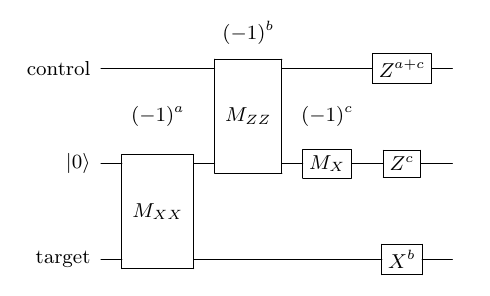
\includegraphics[scale=0.5]{img/cnotMeasureCircuit.png}\\
	\caption{A Quantum Circuit, where $|0\rangle$ is the +1
	eigenstate in $\sigma_z$-basis}
	\label{fig:circuit1}
	\end{center}
\end{figure}
\newpage

In the quantum circuit depicted in figure \ref{fig:circuit1} the input
state can be written as $|\psi_{control}\rangle \otimes |0\rangle 
\otimes |\psi_{target}\rangle$ and the measurement in the first 
timestep can be expressed as $\mathbb{I}\otimes X \otimes X$.\\
To simplify calculation we can write $|\psi_{target}\rangle$ as
$\alpha |+\rangle + \beta |-\rangle$, where $|+\rangle,|-\rangle$ are
the +1 and -1 Eigenstates of the $\sigma_x$-matrix. \\
The input state is thus: 
$|\psi_{control}\rangle \otimes |0\rangle 
\otimes( \alpha |+\rangle + \beta |-\rangle)$.\\
Upon the first measurement, if the measurement result on ancilla $|0\rangle$
is +1, the state becomes:
\begin{equation}
	|\phi^{+}_{t=1}\rangle = |\psi_{control}\rangle \otimes |+\rangle \otimes \alpha |+\rangle
\end{equation}
In this case, a = 0.
If the measurement result is -1, the state becomes:
\begin{equation}
	|\phi^{-}_{t=1}\rangle = |\psi_{control}\rangle \otimes |-\rangle \otimes \beta|-\rangle
\end{equation}
In this case, a = 1.\\
We now write $|\psi_{control}\rangle$ as $\gamma |0\rangle + \delta |1\rangle$
and $|\pm\rangle$ as $\frac{|0\rangle\pm|1\rangle}{\sqrt{2}}$.\\
Upon the second measurement then, if the measurement result on 
the control qubit is +1, and the first ancilla measurement was also +1, the state becomes:\\
\begin{equation}
	|\phi^{++}_{t=2}\rangle = \gamma |0\rangle \otimes |0\rangle \otimes \alpha |+\rangle
\end{equation}
Similarly:
\begin{equation}
	|\phi^{+-}_{t=2}\rangle = -\delta |1\rangle \otimes -|1\rangle \otimes \alpha |+\rangle
\end{equation}
\begin{equation}
	|\phi^{-+}_{t=2}\rangle = \gamma|0\rangle \otimes |0\rangle \otimes \beta|-\rangle
\end{equation}
\begin{equation}
	|\phi^{--}_{t=2}\rangle = -\delta|1\rangle \otimes |1\rangle \otimes \beta|-\rangle
\end{equation}
\\
In X basis, the state of the ancilla will be:\\
\begin{align}
	|\psi_A^{++}\rangle = \frac{|+\rangle+|-\rangle}{\sqrt{2}},
	|\psi_A^{+-}\rangle = \frac{|-\rangle-|+\rangle}{\sqrt{2}}\\
	|\psi_A^{-+}\rangle = \frac{|+\rangle+|-\rangle}{\sqrt{2}},
	|\psi_A^{--}\rangle = \frac{|+\rangle-|-\rangle}{\sqrt{2}}
\end{align}
Therefore, measuring X on the ancilla at t=3 will yield -1 or +1 both with probability
$\frac{1}{2}$ in the ++ and the -+ case, always -1 in the +- case and always +1 in the -- case.
\\
So then the target qubit will be resolved in the following way:
\begin{enumerate}
	\item $Z^{1+1} |\phi^{--}_{t=4}\rangle = -\delta|1\rangle \neq |\phi_{t=0}\rangle ???$
\end{enumerate}


\newpage
Meanwhile, in the Heisenberg picture we focus on the time-evolution of Operators:
\begin{equation}
	H = H(t)
\end{equation}
By specifically looking at the time evolution of those operators
to which the states in the system's input state space are 
eigenstates, we can figure out a systems output state space via:
\begin{equation}
	Circuit(\psi)=Circuit(H)\psi
\end{equation}
